\documentclass{article}

\usepackage{graphicx}
\usepackage[margin=1in]{geometry}
\usepackage[hidelinks]{hyperref}
\usepackage{pgfplots}
\usepackage{multicol}
\usepackage{caption}

\title{HLA draft (to be included in ccsc paper)}
\date{October 11, 2016}
\author{Christopher Silva}

\makeatletter
\renewcommand\thesection{}
\renewcommand\thesubsection{\@arabic\c@subsection.}
\makeatother

\renewcommand{\thesubsubsection}{\alph{subsubsection}.}

\begin{document}
	\maketitle
	\pagenumbering{gobble}
	\newpage
	\pagenumbering{arabic}
	\begin{multicols}{2}
		High-Level Architecture(HLA) is an architecture that allows many distributed simulation systems to work together seamlessly. \\
		There are five parts to a HLA system:
		\begin{itemize}
			\item Runtime Infrastructure(RTI) - Software that provides HLA services.
			\item Federate - A simulation system that connects to the RTI.
			\item Federation Object Model(FOM) - A description of data exchanges in a federation.
			\item Federation - All of the federates along with the RTI and the FOM they use.
			\item Federation Execution - An instance of the federation.
		\end{itemize}
		HLA uses a publish/subscribe methodology for information services. This means that a federate "publishes" certain data and "subscribes" to other data. To publish data a federate sends it to the RTI. To receive subscribed data a federate will receive a callback from the RTI anytime the subscribed data is updated. \\
		
		\captionof{figure}{MWSU Satellite publish/subscribe listing.}\label{interactions}
		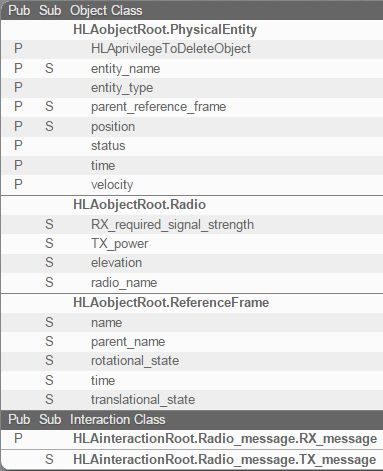
\includegraphics[width=\columnwidth]{interactions.png}
		
		The FOM contains descriptions of the Objects, Interactions, and Data Types that federates will use in a federation. Because of this all federates must agree on which FOMs to use. This is arguably the most important part of the HLA standard; it ensures that the designers of each federate communicate in order to come to an agreement on not just the FOM, but on other aspects such as the overall goal of the simulation.
		
		\captionof{figure}{FOMs used in SEE 2016.}\label{fom}
		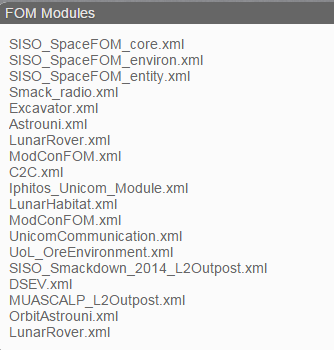
\includegraphics[width=\columnwidth]{fom.png}
		
		The recommended representation for a federation is call a "lollipop" diagram. 
		
		\captionof{figure}{SEE 2016 participants lollipop diagram.}\label{lollipop}
		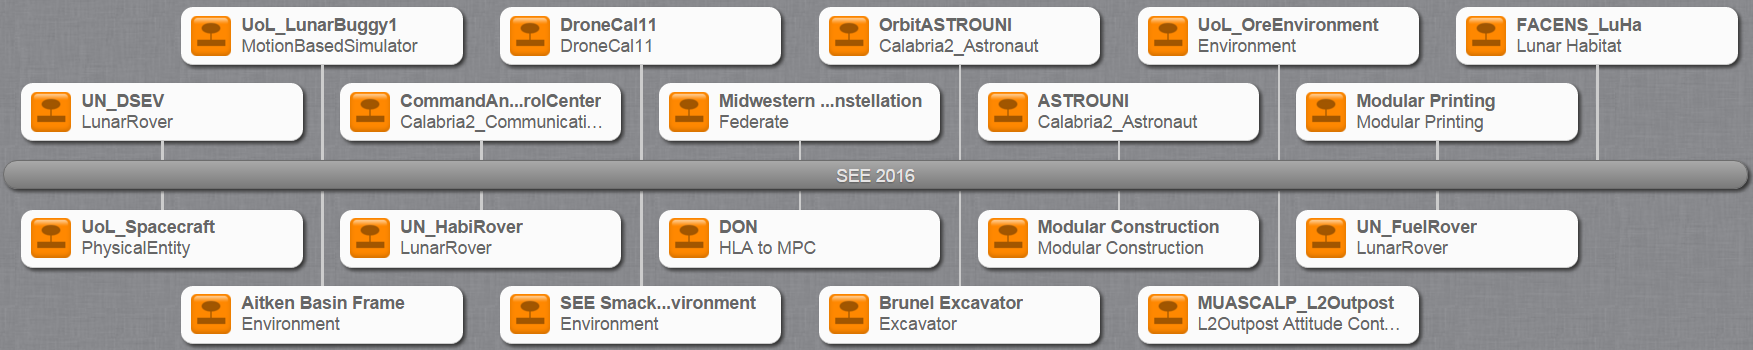
\includegraphics[width=\columnwidth]{lollipop.png}
		
		
		
	\end{multicols}
\end{document}